\documentclass{Report}
\usepackage[utf8]{inputenc}
\usepackage{relsize}
\usepackage[backend=bibtex,style=verbose-trad2]{biblatex}
\usepackage{graphicx}
\usepackage{listings}
\usepackage{subfigure}
\bibliography{COMP120} 

\newcommand{\subtitlerelsize}{1} %relative size: integer value
\newcommand{\subtitlelinesep}{0.2em} %line separation: a LaTeX length

\title{Colour Blindness Report\\[\subtitlelinesep]\smaller[\subtitlerelsize]{}COMP120 Tinkering Graphics}
\author{James Arthur}
\date{October 2019}

\begin{document}

\maketitle

\section{Introduction}
Colour Blindness or Colour Deficiency, affects 1 in 12 men and 1 in 200 women across the world.\autocite{CBA} This means that there are 3 million people in the UK that are colourblind. Colour Blindness is usually a genetic fault on chromosomes, the overpowering bias towards males in the figures is due to the most common form of Colour Blindness, red-green, being tranferred through the X Chromosome.\autocite{copsin} On the opposing side, an injury can induce Colour Blindness, these include: Eye Diseases (Gluacoma and Macular Degeneration), Brain and Nervous System Diseases (Alzheimers or multiple Sclerosis) or alternatively there are some types of medicines with side effects as Colour Blindness, such as Planquenil, a rheumatiod arthritis medicine. \autocite{NIH}\\\\

There are many different types of Colour Blindness, I shall strive to create an algorithm to simulate every type of Colour Blindness. The types depend on how many of the cone types are defficient.  You have Anomalous Trichromacy in which one type of cone is defficient, Dichromacy is where two of the cones are completely defficient and Monochromacy where the patient sees no colour, with usually greyscale vision.\autocite{Types} It can also be noted that some people describe that Colour Blindness as the confusion of different colours, this is seen in some of my code. \autocite{NHS} \\\\

In this report I shall set out my work to produce an a couple of algorithms to simulate all the different types of Colour Blindness, they have all be produced in PyCharm 2019.2.3 using PyGame 1.9.4 in Python 3.7. The image that I shall be using is one that I have taken, it requires no citing.

\newpage

\section{Anomalous Trichromacy}
\subsection{Protanomaly}

Protanomaly is reduced sensitivity to red light.\autocite{Types}
\subsubsection{Code}
\lstinputlisting{./ColourBlindness/Trichromatanomaly/protanomaly.py}

\newpage

\subsubsection{Results}
\begin{figure}[h!]
  \centering
  \caption{Original Picture}
  \includegraphics[width=0.5\textwidth]{Lizard}
  \centering
  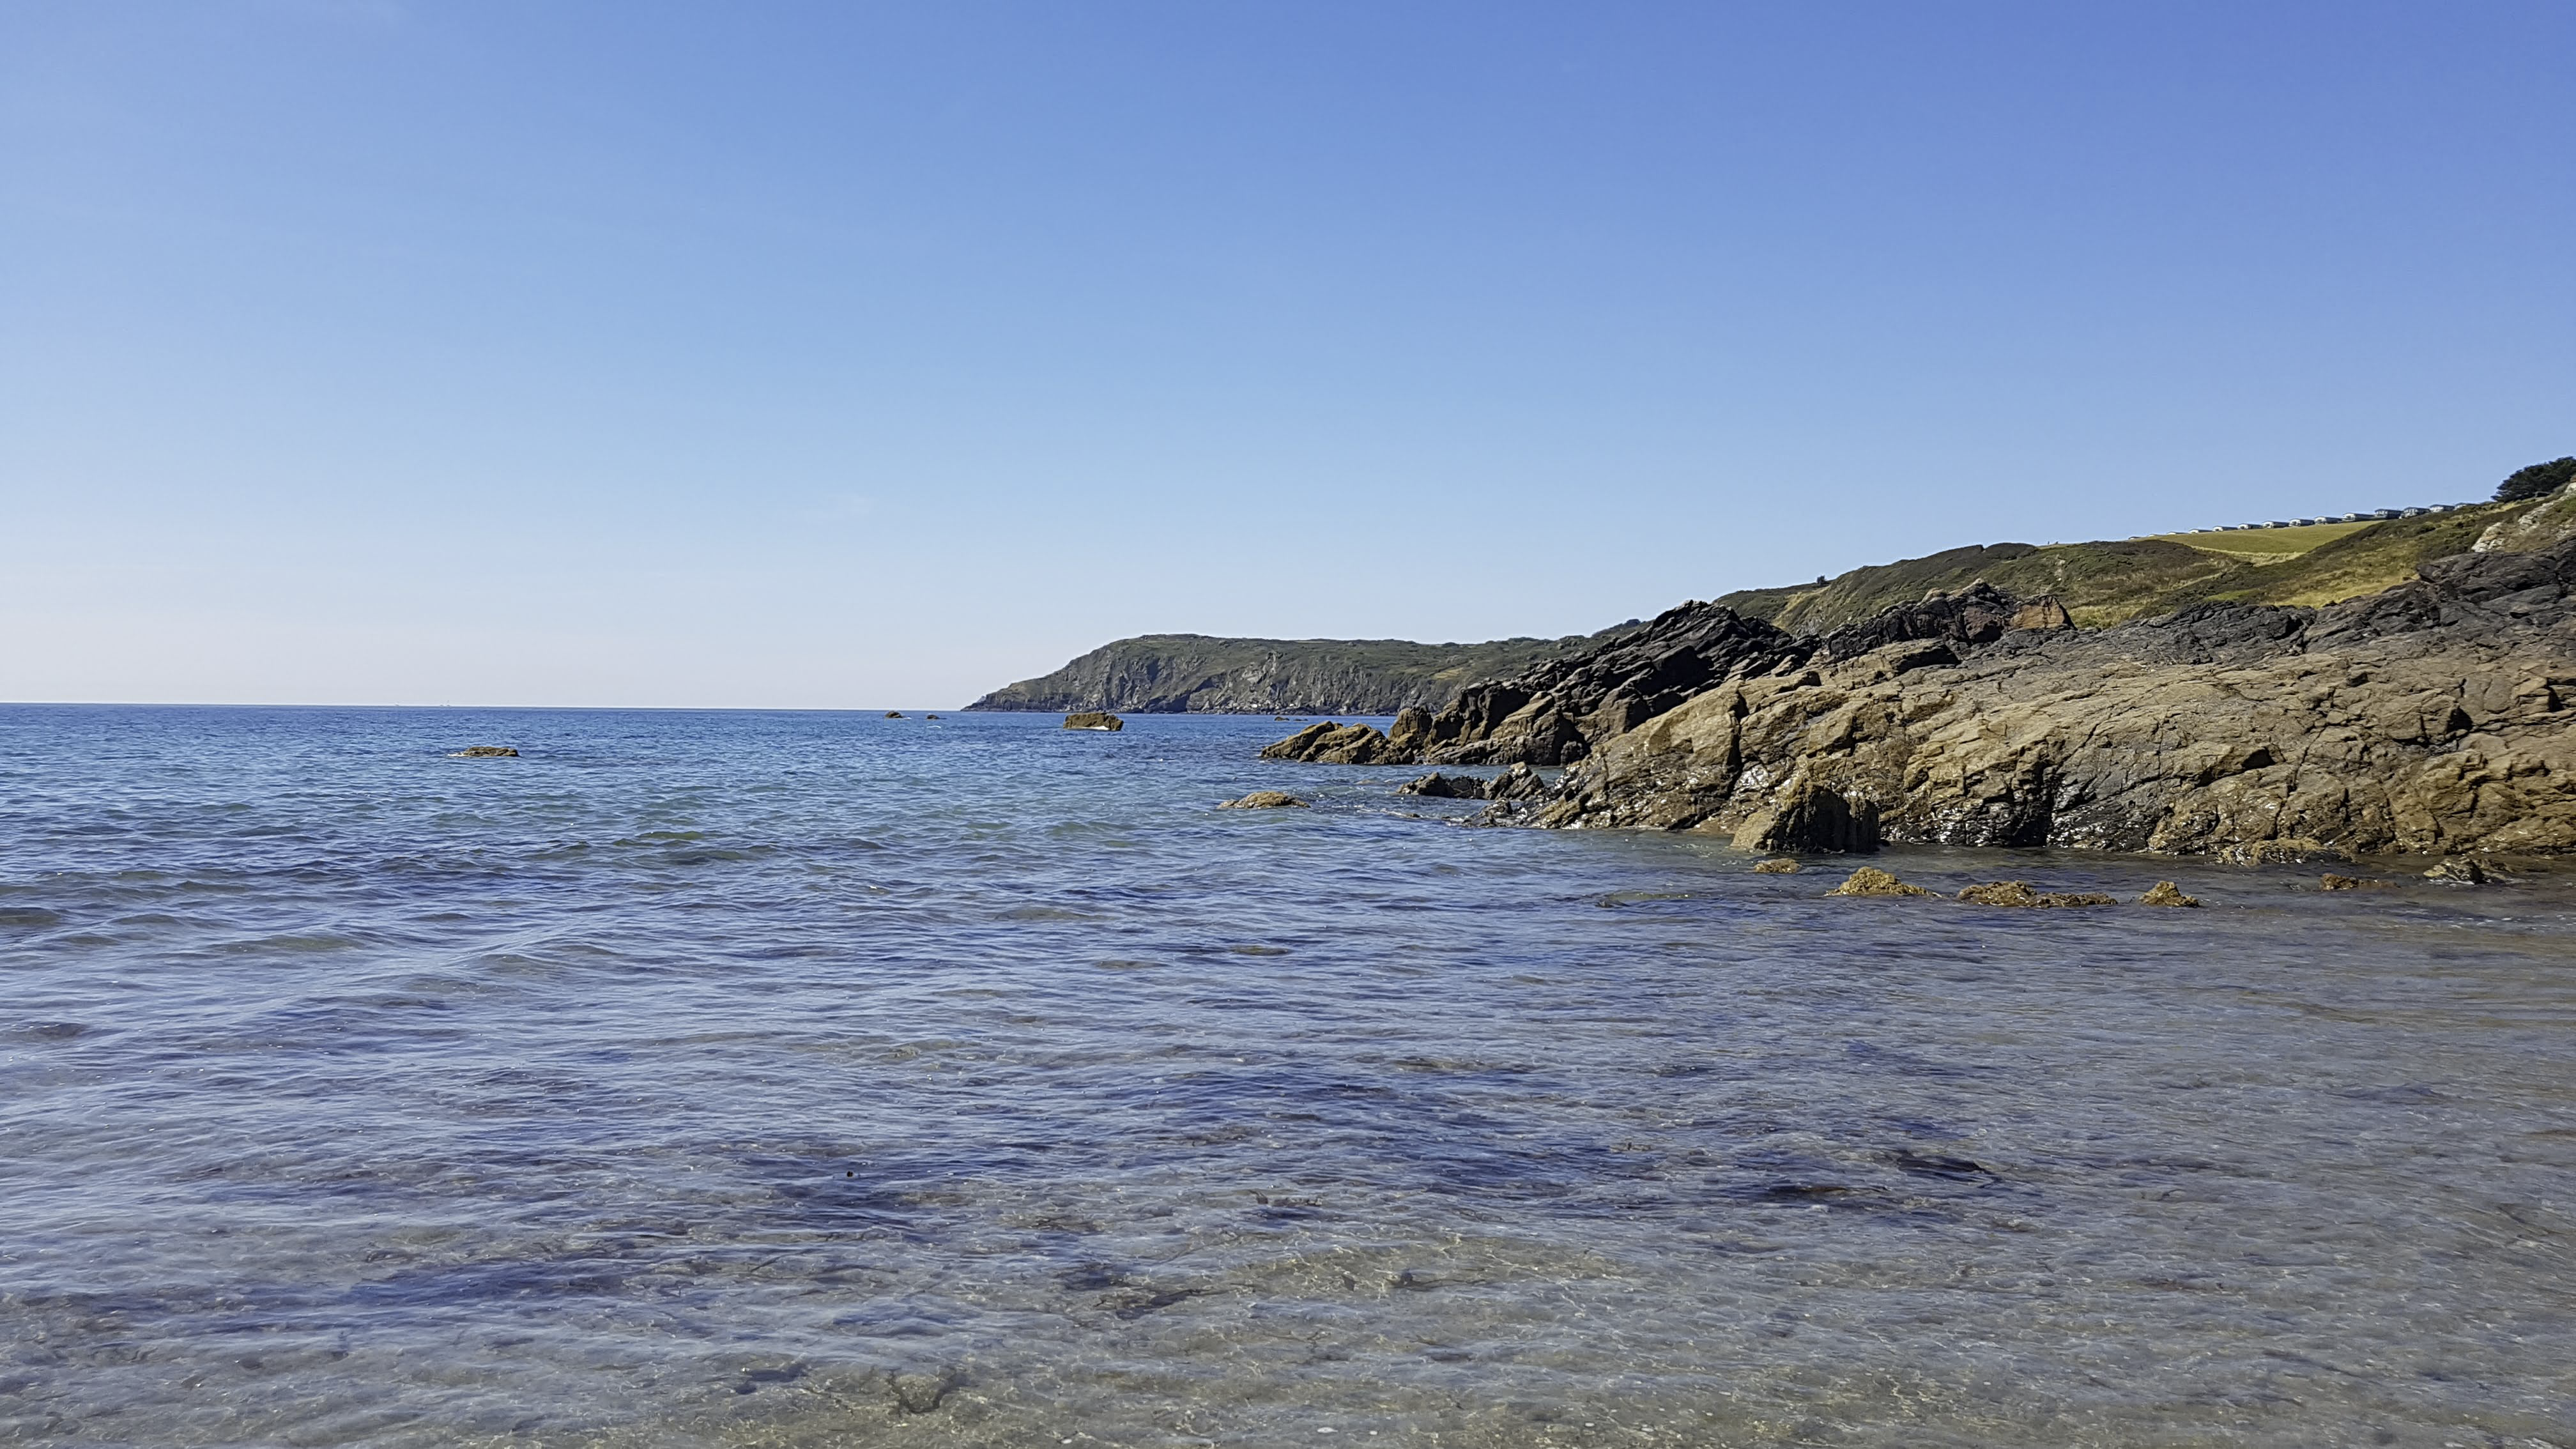
\includegraphics[width=0.5\textwidth]{./ColourBlindness/Trichromatanomaly/protanomaly.png}
  \caption{Protanomaly version}
\end{figure}

\newpage

\subsection{Dueteranomaly}

Dueteranomaly is reduced sensitivity to green light. \autocites{Types}
\subsubsection{Code}
\lstinputlisting{./ColourBlindness/Trichromatanomaly/deuteranomaly.py}

\newpage

\subsubsection{Results}
\begin{figure}[h!]
  \centering
  \caption{Original Picture}
  \includegraphics[width=0.5\textwidth]{Lizard}
  \centering
  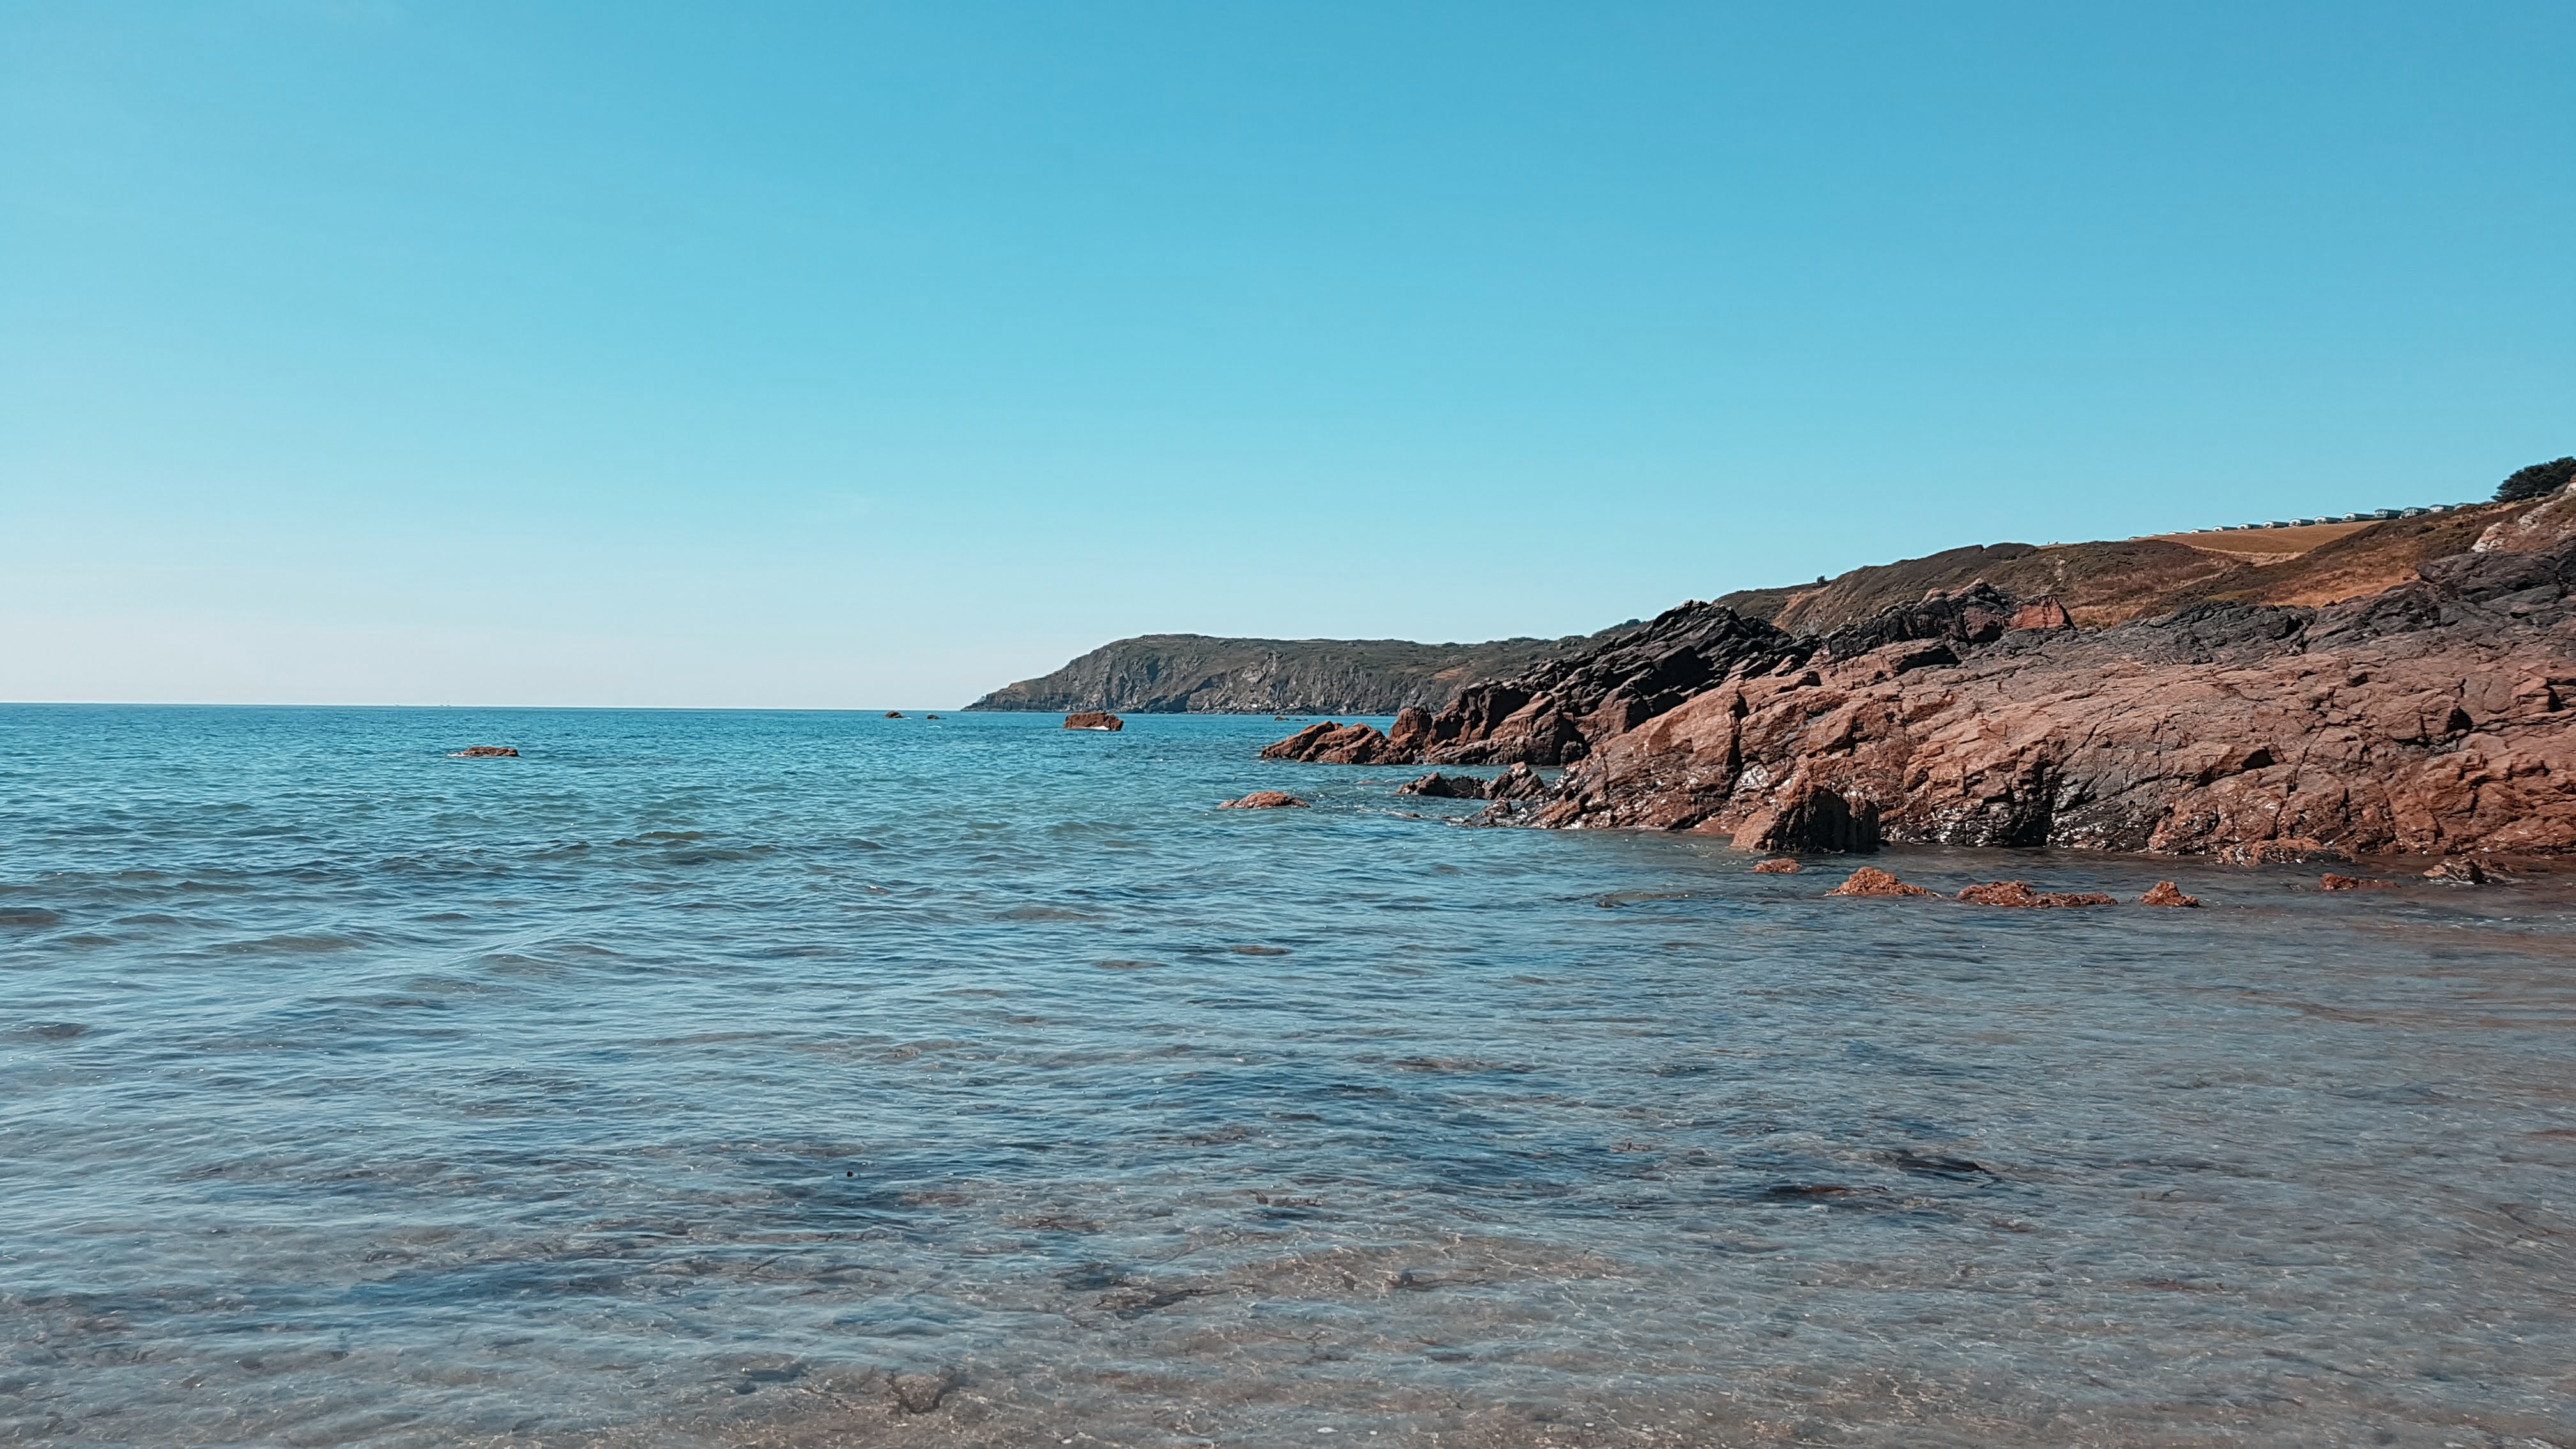
\includegraphics[width=0.5\textwidth]{./ColourBlindness/Trichromatanomaly/deuteranomaly.png}
  \caption{Dueteranomaly version}
\end{figure}

\newpage

\subsection{Tritanomaly}

Tritanomaly is reduced sensitivity to blue light. \autocites{Types}
\subsubsection{Code}
\lstinputlisting{./ColourBlindness/Trichromatanomaly/tritanomaly.py}

\newpage

\subsubsection{Results}
\begin{figure}[h!]
  \centering
  \caption{Original Picture}
  \includegraphics[width=0.5\textwidth]{Lizard}
  \centering
  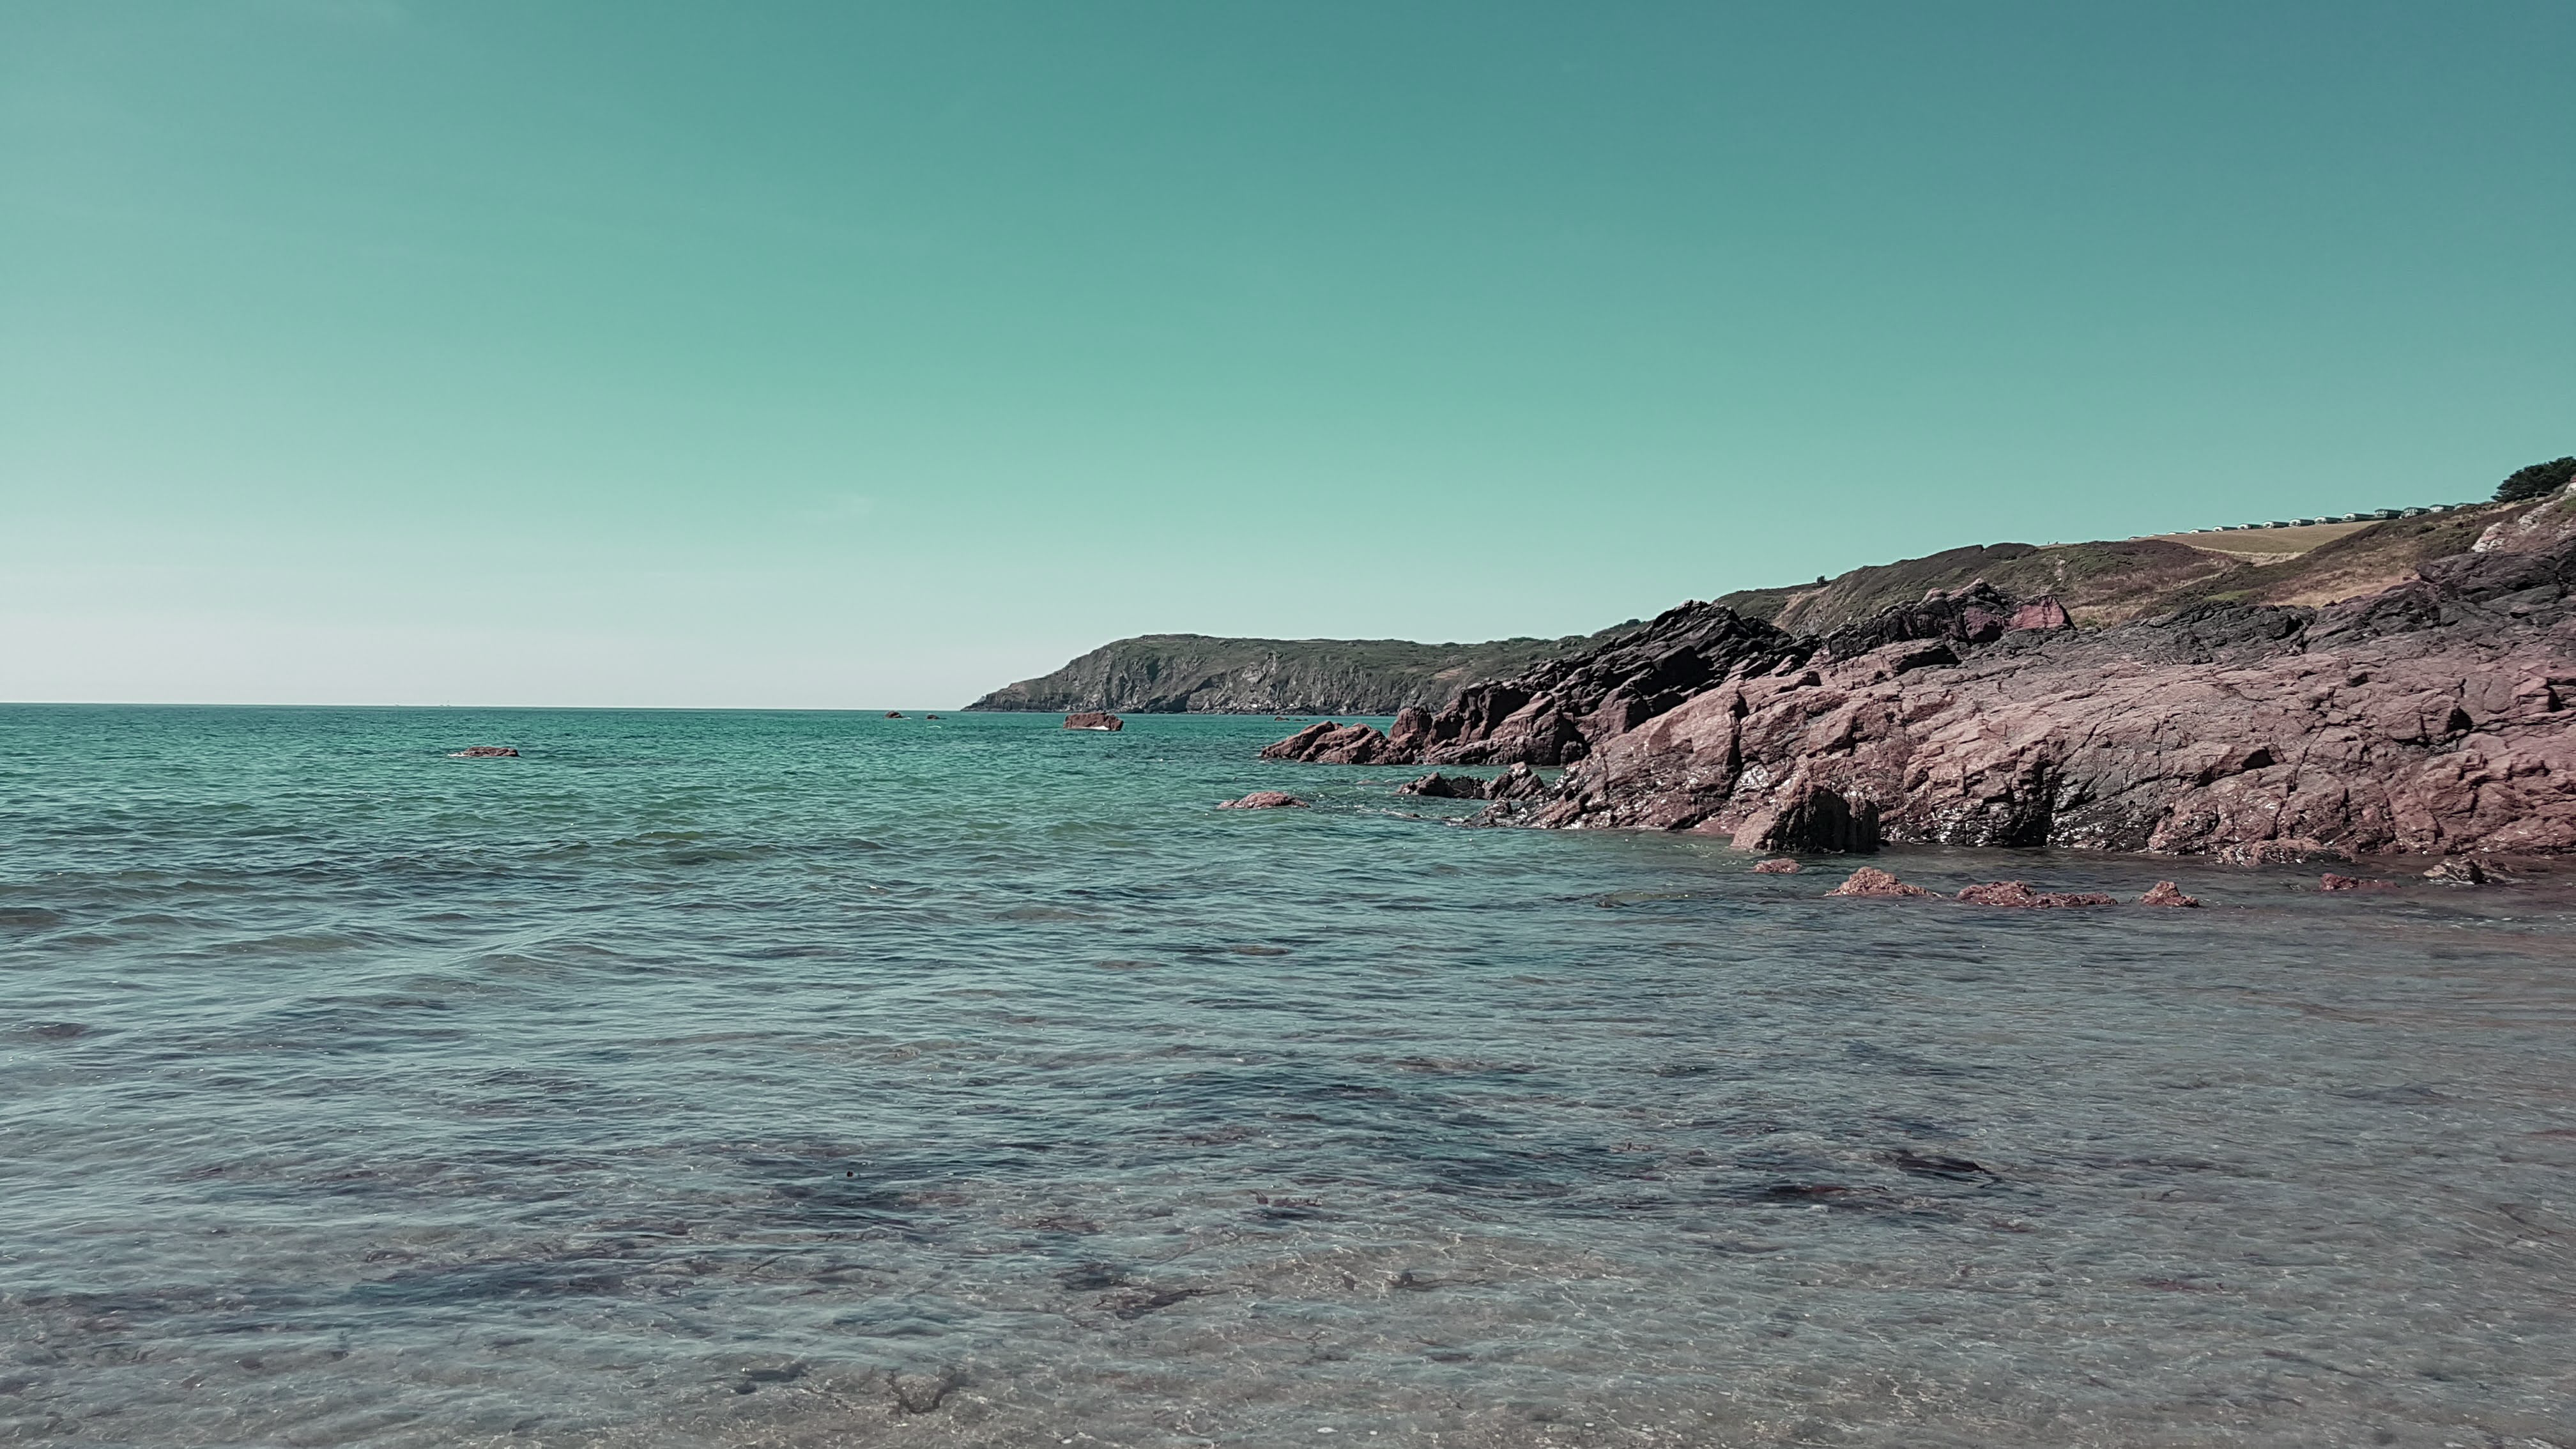
\includegraphics[width=0.5\textwidth]{./ColourBlindness/Trichromatanomaly/tritanomaly.png}
  \caption{Tritanomaly version}
\end{figure}

\newpage

\subsection{Dueteropia}

Dueteropia is no sensitivity to green light. \autocites{Types}
\subsubsection{Code}
\lstinputlisting{./ColourBlindness/Dichromat/Dueteropia.py}

\newpage

\subsubsection{Results}
\begin{figure}[h!]
  \centering
  \caption{Original Picture}
  \includegraphics[width=0.5\textwidth]{Lizard}
  \centering
  \includegraphics[width=0.5\textwidth]{./ColourBlindness/Dichromat/Deuteropia.jpg}
  \caption{Dueteropia version}
\end{figure}

\newpage

\subsection{Protanopia}

Protanopia is no sensitivity to red light. \autocites{Types}
\subsubsection{Code}
\lstinputlisting{./ColourBlindness/Dichromat/Protanopia.py}

\newpage

\subsubsection{Results}
\begin{figure}[h!]
  \centering
  \caption{Original Picture}
  \includegraphics[width=0.5\textwidth]{Lizard}
  \centering
  \includegraphics[width=0.5\textwidth]{./ColourBlindness/Dichromat/Protanopia.jpg}
  \caption{Protanopia version}
\end{figure}

\newpage

\subsection{Tritanopia}

Tritanopia is no sensitivity to blue light. \autocites{Types}
\subsubsection{Code}
\lstinputlisting{./ColourBlindness/Dichromat/Tritanopia.py}

\newpage

\subsubsection{Results}
\begin{figure}[h!]
  \centering
  \caption{Original Picture}
  \includegraphics[width=0.5\textwidth]{Lizard}
  \centering
  \includegraphics[width=0.5\textwidth]{./ColourBlindness/Dichromat/Tritanopia.jpg}
  \caption{Tritanopia version}
\end{figure}

\newpage

\subsection{Monochromat}

Monochromat is no sensitivity to any coloured light. \autocites{Types}
\subsubsection{Code}
\lstinputlisting{./ColourBlindness/Monochromat/monochromat.py}

\newpage

\subsubsection{Results}
\begin{figure}[h!]
  \centering
  \caption{Original Picture}
  \includegraphics[width=0.5\textwidth]{Lizard}
  \centering
  \includegraphics[width=0.5\textwidth]{./ColourBlindness/Monochromat/Monochromat.jpg}
  \caption{Monochromat version}
\end{figure}

\newpage

\printbibliography

\end{document}